\chapter{Las cónicas de Apolonio}

\index{Cónicas}
\index{Elipse}
\index{Hipérbola}
\index{Parábola}
Las \textbf{cónicas} son aquellas curvas que se obtienen al cortar un cono
circular con un plano. Las cónicas son entonces hipérboles, elipses o
parábolas. Hoy sabemos que podemos representar cónicas mediante ecuaciones. La expresión 
\[
	\frac{x^2}{a^2}-\frac{y^2}{b^2}=1
\]
es la ecuación de una hipérbola, la expresión 
\[
	\frac{x^2}{a^2}+\frac{y^2}{b^2}=1
\]
es la ecuación de una elipse y la expresión 
\[	
	y=ax^2
\]
es la ecuación de una parábola. 

Se cree que las cónicas fueron inventadas por Menecmo en épocas de Alejandro
Magno. Originalmente Menecmo utilizó las cónicas para reformular (y en algún
sentido resolver) el famoso problema de la duplicación del cubo. En nuestra
notación, el problema de la duplicación del cubo puede reformularse como el
problema de encontrar la intersección de la parábola $y=\frac12x^2$ con la
hipérbola $xy=1$, ya que esto implica encontrar un $x$ tal que $x^3=2$. Los
griegos aparentemente nunca discutieron sobre los intrumentos que necesarios
para dibujar cónicas, aunque sí aceptaron la solución propuesta por Menecmo.
Las ideas de Menecmo sugieren la existencia de un instrumento que resulta ser
una generalización del compás, este instrumento, en forma independiente,
aparece en la matemática árabe del siglo XI. 

El estudio profundo de las cónicas y sus propiedades fhe hecho por Apolonio,
alrededor del año 200 a. C.  Dado que no disponían del álgebra, los griegos no
pudieron estudiar sistemáticamente curvas de grado superior. Sin embargo, sí
fueron capaces de estudiar ciertas curvas particulares sin necesidad de
utilizar ecuaciones que las definan. Un ejemplo notable es la cisoide de
Diocles. 

En 1609 Kepler descubrió que las órbitas planetarias son elipses. Este hecho fue
explicado en 1687 por la teoría gravitatoria de Newton. 

\section*{Algunas curvas algebraicas}

\index{Curva algebraica}
Como los griegos no disponían del álgebra, no pudieron profundizar sus
conocimientos sobre curvas, aunque sí pudieron estudiar algunas curvas
algebraicas particulares. Una curva algebraica es una curva dada por los ceros
de un polinomio de dos variables.  Para una digresión histórica sobre la teoría
de curvas algebraicas, referimos al primer capítulo del libro de Brieskorn y
Kn\"{o}rrer \cite{MR2975988}.

\index{Cisoide de Diocles}
Veamos algunos ejemplos de las curvas consideradas en la matemática griega. 
Diocles concibió la curva de hoy conocemos como \emph{cisoide de Diocles} y observó que
esta curva permite duplicar el cubo. Podemos ver una representación gráfica de
esta curva en la figura~\ref{fig:cisoide}. En nuestra notación, esta curva
está representada por la ecuación
\[
	y^2(1+x)=(1-x)^3.
\]

\begin{figure}
   \centering
   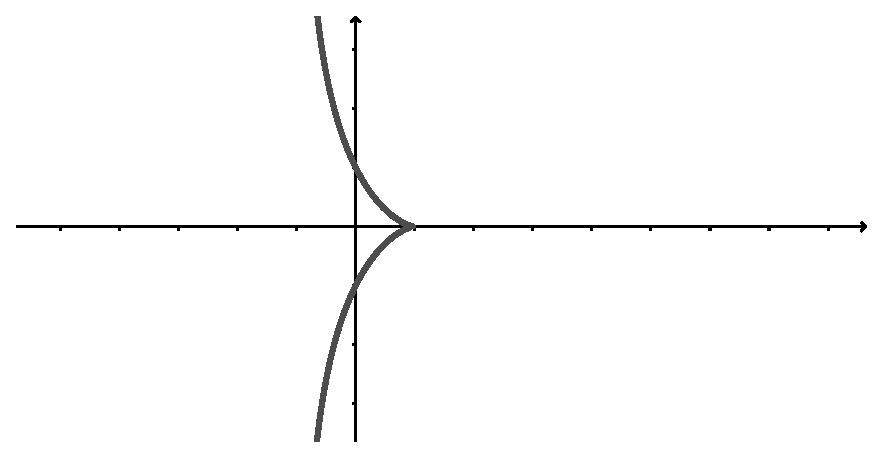
\includegraphics[scale=0.3]{images/cisoide}
   \caption{La cisoide de Diocles.}
   \label{fig:cisoide}
\end{figure}

\index{Toro}
\index{Secciones espíricas}
Los matemáticos griegos conocían algunas superficies. Una de las superficies
que estudiaron es el toro, que es una superficie de revolución tal como la que
podemos ver en la figura~\ref{fig:toro}. 

\begin{figure}
   \centering
   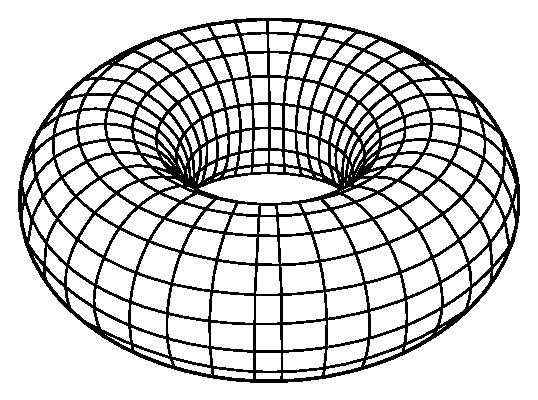
\includegraphics[scale=0.3]{images/toro}
   \caption{El toro.}
   \label{fig:toro}
\end{figure}

Perseo estudió las curvas que se obtienen al cortar el toro
con planos paralelos al eje de rotación, estas curvas se conocen como 
\emph{curvas espíricas}. La ecuación de estas curvas está dada por
\[
	(x^2+y^2)^2=dx^2+ey^2+f.
\]

\begin{figure}
   \centering
   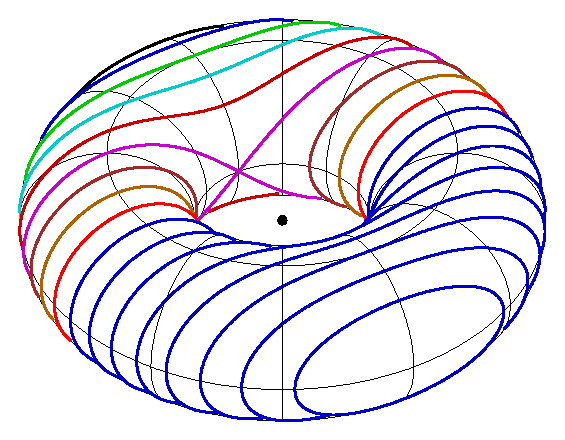
\includegraphics[scale=0.3]{images/spiric}
   \caption{Las curvas espíricas.}
   \label{fig:spiric}
\end{figure}



\index{Lemniscata de Bernoulli}
Algunas de estas curvas fueron redescubiertas en el
siglo XVII gracias a la geometría analítica de Descartes. Un ejemplos notable 
el de la \emph{lemniscata de Bernoulli}, descubierta en 1694 por Jakov Bernoulli. La ecuación 
de esta curva es 
\[
	(x^2+y^2)^2=x^2-y^2
\]
y podemos ver una representación gráfica en la figura~\ref{fig:lemniscata}.

\begin{figure}
   \centering
   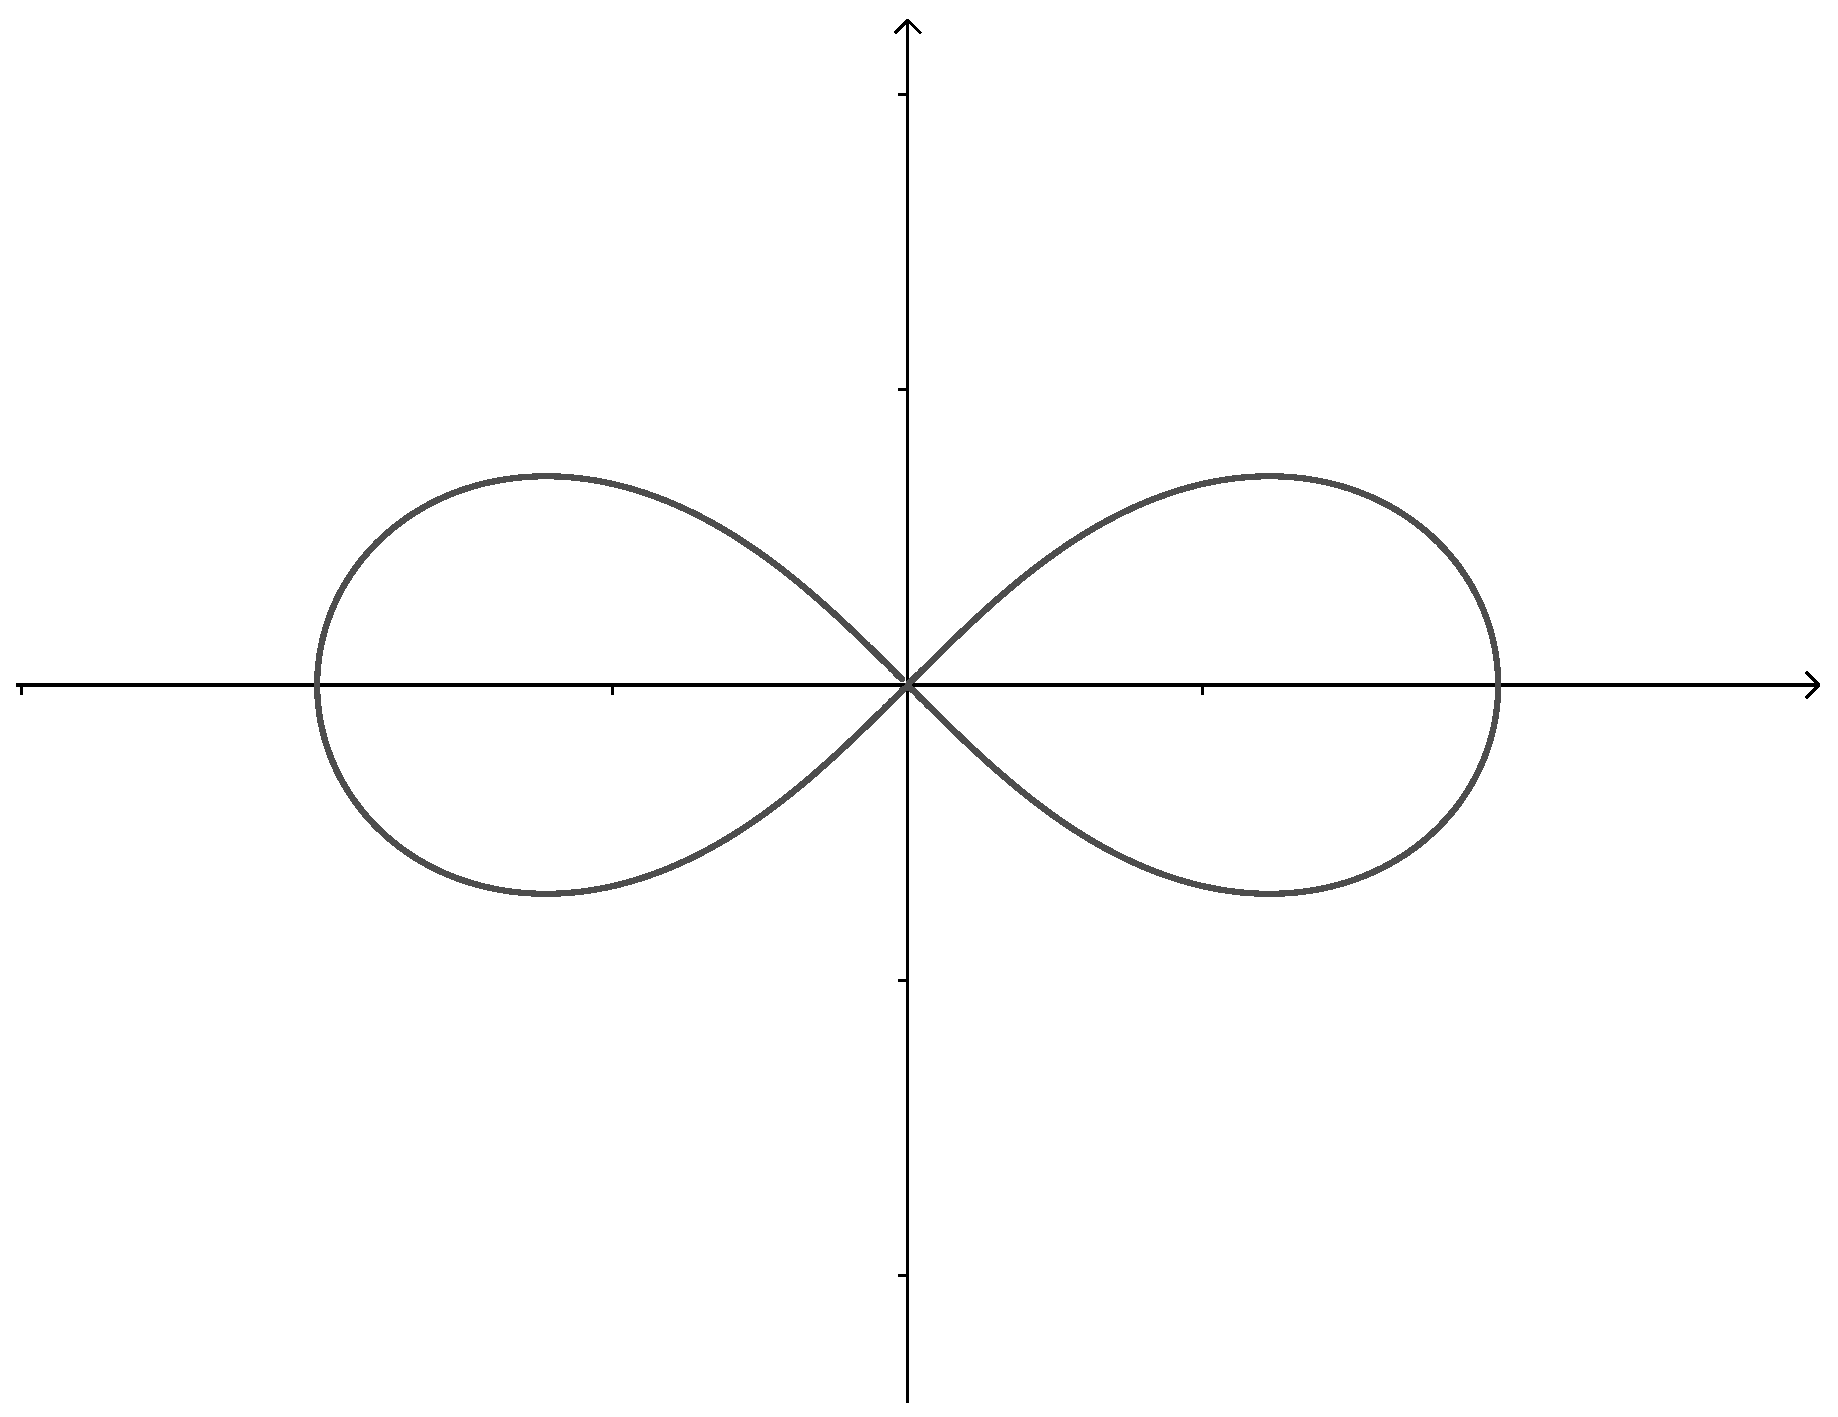
\includegraphics[scale=0.2]{images/lemniscata}
   \caption{La Lemniscata de Bernourlli.}
   \label{fig:lemniscata}
\end{figure}
 
\index{Óvalos de Cassini}
Otro ejemplo es el de los \emph{óvalos de Cassini}, que vemos en la
figura~\ref{fig:Cassini}, y que el astrónomo propuso para reemplazar a las
elipses de Kepler que describen las órbitas planetarias. 

\index{Epiciclos de Ptolomeo}
\index{Cardioide}
Otra familia de curvas estudiadas por la matemática griega es la de los
epiciclos de Ptolomeo. Estas curvas también tienen sus orígines en la
astronomía, ya que eran los candidatos naturales a describir las órbitas
planetarias. Un ejemplo de estas curvas es el de la \emph{cardioide} de ecuación
\[
	(x^2+y^2-1)^2=4( (x-1)^2+y^2)
\]
que vemos en la figura~\ref{fig:cardioide}.
